\documentclass[letterpaper]{article} % DO NOT CHANGE THIS
\usepackage[submission]{aaai23}  % DO NOT CHANGE THIS
\usepackage{times}  % DO NOT CHANGE THIS
\usepackage{helvet}  % DO NOT CHANGE THIS
\usepackage{courier}  % DO NOT CHANGE THIS
\usepackage[hyphens]{url}  % DO NOT CHANGE THIS
\usepackage{graphicx} % DO NOT CHANGE THIS
\urlstyle{rm} % DO NOT CHANGE THIS
\def\UrlFont{\rm}  % DO NOT CHANGE THIS
\usepackage{natbib}  % DO NOT CHANGE THIS AND DO NOT ADD ANY OPTIONS TO IT
\usepackage{caption} % DO NOT CHANGE THIS AND DO NOT ADD ANY OPTIONS TO IT
\usepackage{subcaption} % DO NOT CHANGE THIS AND DO NOT ADD ANY OPTIONS TO IT
\frenchspacing  % DO NOT CHANGE THIS
\setlength{\pdfpagewidth}{8.5in} % DO NOT CHANGE THIS
\setlength{\pdfpageheight}{11in} % DO NOT CHANGE THIS
\usepackage[ruled,vlined,linesnumbered]{algorithm2e}
\usepackage{xcolor}
\setcounter{secnumdepth}{2} %May be changed to 1 or 2 if section numbers are desired.
\usepackage{xspace}
\newcommand{\plan}[1]{{\textcolor{blue}{[Plan: #1]}}}
\newcommand{\blocked}{\textit{blocked}}
\newcommand{\unblocked}{\textit{unblocked}}
\newcommand{\unknown}{\textit{b}|\textit{u}}
\newcommand{\assumeObs}{\textbf{AssumeObs}}
\newcommand{\toplan}{\textit{tree2plan}}
\newcommand{\po}{PO\xspace}
\newcommand{\pos}{POs\xspace}
\newcommand{\cons}{\textit{cons}}
\newcommand{\const}{\textit{Const}}
\newcommand{\pbad}{\ensuremath{p_{\textit{bad}}}}
\newcommand{\tuple}[1]{\ensuremath{\left \langle #1 \right \rangle }}
\newcommand{\guy}[1]{{\textcolor{red}{[Guy: #1]}}}
\newcommand{\Bar}[1]{{\textcolor{orange}{[Bar: #1]}}}
\newcommand{\roni}[1]{{\textcolor{green}{[Roni: #1]}}}
\newcommand{\commentout}[1]{}
\usepackage{amsthm,amsmath}
\newtheorem{exmp}{Example}
\newtheorem{theorem}{Theorem}
\newtheorem{observation}{Observation}
\newtheorem{corollary}{Corollary}
\newtheorem{lemma}{Lemma}
\newtheorem{definition}{Definition}
\usepackage{newfloat}
\usepackage{listings}
\DeclareCaptionStyle{ruled}{labelfont=normalfont,labelsep=colon,strut=off} % DO NOT CHANGE THIS
\lstset{%
	basicstyle={\footnotesize\ttfamily},% footnotesize acceptable for monospace
	numbers=left,numberstyle=\footnotesize,xleftmargin=2em,% show line numbers, remove this entire line if you don't want the numbers.
	aboveskip=0pt,belowskip=0pt,%
	showstringspaces=false,tabsize=2,breaklines=true}
\title{Multi Agent Path Finding Under Obstacle Uncertainty}
\author{
    Written by AAAI Press Staff\textsuperscript{\rm 1}\thanks{With help from the AAAI Publications Committee.}\\
    AAAI Style Contributions by Pater Patel Schneider,
    Sunil Issar,\\
    J. Scott Penberthy,
    George Ferguson,
    Hans Guesgen,
    Francisco Cruz\equalcontrib,
    Marc Pujol-Gonzalez\equalcontrib
}
\affiliations{
    \textsuperscript{\rm 1}Association for the Advancement of Artificial Intelligence\\
    1900 Embarcadero Road, Suite 101\\
    Palo Alto, California 94303-3310 USA\\
    publications23@aaai.org
}
\iffalse
\title{My Publication Title --- Single Author}
\author {
    Author Name
}
\affiliations{
    Affiliation\\
    Affiliation Line 2\\
    name@example.com
}
\fi
\iffalse
\title{My Publication Title --- Multiple Authors}
\author {
    First Author Name,\textsuperscript{\rm 1}
    Second Author Name, \textsuperscript{\rm 2}
    Third Author Name \textsuperscript{\rm 1}
}
\affiliations {
    \textsuperscript{\rm 1} Affiliation 1\\
    \textsuperscript{\rm 2} Affiliation 2\\
    firstAuthor@affiliation1.com, secondAuthor@affilation2.com, thirdAuthor@affiliation1.com
}
\fi
\usepackage{bibentry}
\begin{document}
\maketitle
\begin{abstract}
In multi-agent path finding (MAPF), several agents must move from their current positions to their target positions without colliding. In this paper we focus on a MAPF setting where a set of obstacles may exist at known positions. When an agent is close to such a position, it can sense whether the obstacle exists, and plan accordingly. In this setting, the solution for an agent is a plan tree, branching on the observations.
While we focus here on centralized planning, we consider two modes of execution, where the agents share information concerning observed obstacles during execution, and where no such communication is allowed.
We study two optimization criteria --- optimizing for the best case, and optimizing for the worst case.
For conflict resolution, we use the CBS method, adapting constraints to be conditioned on observations.
We provide experiments demonstrating how our approach scales up with respect to the problem size, number of agents, and the amount of possible obstacles.
\end{abstract}
\section{Introduction}
In multi agent path finding (MAPF), we must plan for several agents to move from their current positions to some target positions without colliding \cite{stern2019multi}. This is an important task with numerous real world applications, ranging from the movement of robotic arms, through robots in automated warehouses, to autonomous cars.
Research in MAPF has mainly focused on the classical case, where we have full observability over the environment. That is, MAPF researchers often assume that we know, in advance, which cells of a grid that we navigate in will be blocked. However, in many practical robotic applications, the robot can only identify obstacles through sensors, typically only within some proximity \cite{lenser2003visual}.
In this paper we extend the MAPF problem to partial observability over obstacles. We assume that while some obstacles (e.g. walls), are known in advance, other obstacles (e.g. heavy objects or closed doors) can only be sensed once the agent reaches the proximity of the obstacles. We call this problem MAPF under obstacle uncertainty (MAPFOU).
Solving MAPFOU problems is harder than classical MAPF problems (CMAPF), because the plan may require different solutions given different obstacles. This can be formalized a  plan tree \cite{hoffmann2005contingent}, branching on obstacle observations. These plan trees can be exponential in the number of uncertain obstacles.
While we assume centralized planning, we investigate two cases for plan execution. First, execution can be centralized, that is, all agents share their observations. Hence, the plan tree of one agent can branch on the observations of other agents. In many cases, however, communication is impossible, and each agent must rely only on its own observations, leading to decentralized execution.
To avoid collisions, one may compute a plan jointly, that is, searching in the space of joint plans, avoiding movements that lead to a collision. However, planning for several agents together increases the search space exponentially. Hence, CMPAF research focuses on suggesting methods to plan for each agent individually, while maintaining safe (collision-free) plans. We follow their footsteps here, focusing on methods that plan for each agent individually.
CMAPF research often requires optimal plans \cite{stern2019multi}. We suggest two different optimality criteria, focusing on optimizing either for the best case, where all obstacles do not exist, or the worst case, where all obstacles exist.
We report a set of experiments, analyzing the performance of our algorithms over different settings, with respect to the grid size, the number of agents, and the amount of obstacles.
\section{Background and Related Work}
We now review relevant background on multi-agent path finding problems, the CBS algorithm, and contingent planning under partial observability and sensing actions.
\subsubsection{Classic MAPF Problem}
A \emph{classical multi agent path-finding problem} (CMAPF) \cite[e.g.][]{stern2019multi} for $k \geq 2$ agents is a tuple $\langle G,s,t \rangle$
where $G = (V, E)$ is an undirected graph, and $s,t$ are lists of vertexes. $s = [s_1, s_2, ..., s_k], t = [t_1, t_2, ..., t_k]$ define source and target vertexes for each agent, i.e., $s_i$ is the initial vertex where agent $i$ begins, and $t_i$ is the target vertex where agent $i$ should arrive.
Time is discrete, and at every time step, each
agent either moves to a neighbor vertex, or waits. Actions can be defined as a function $a : V \rightarrow V$ such that $a_{i,j}$ moves the agent from $v_i$ to $v_j$. The set of actions is $A=\{a_{i,j}:(v_i, v_j) \in E\}$. In addition, for every vertex $v_i$, $a_{i,i}$ denotes waiting at $v_i$ for one step.
A classical \emph{single-agent plan} for agent $i$ is a sequence of actions $\pi = (a_1, . . ., a_n)$, in $A$, such that $a_1=a_{s_i,j}$, and $a_n=a_k,t_i$.
A pair single-agent plans $\pi^i$ and $\pi^j$ is said to have a \emph{conflict} if they plan to occupy the same vertex at the same time. This is called a vertex conflict~\cite{stern2019multi}. We leave discussion of other conflict types to future research.
A \emph{solution} to a CMAPF problem is a set of classical single-agent plans $\Pi = \{ \pi^i \}_{i=0}^k $, one for each agent, such that all pairs of single-agent plans do not conflict.
We assume that agents that arrive at their target positions exit the graph, and hence, cannot participate in additional conflicts. Extending our algorithms to agents that remain in the graph until all agents arrive at their target is straightforward.
A solution to a CMAPF problem can be optimal with respect to a given objective function.
Two common objective functions in the CMAPF literature are \emph{makespan} --- the amount of time-steps until
the last agent reaches its target locations, and \emph{sum of costs} (SOC) --- the total amount of actions required by all agents to reach their target location. In this paper we focus on the SOC, but conversion to makespan would not require a significant change.
As with other multi-agent problems, during planning, MAPF problems can be either \emph{distributed} or \emph{centralized}. In a distributed setting, each agent plans independently, and information sharing must be done through pre-designed communication protocols, that may incur additional cost. In a \emph{centralized} setting, we assume a single central computing power which plans and searches for a solution for all agents.
In this paper we focus on centralized planning. However, in our case, one must consider whether the execution is also centralized, i.e., whether agents share information over the obstacles they observe while executing the plans.
\begin{figure}[t]
    \centering
      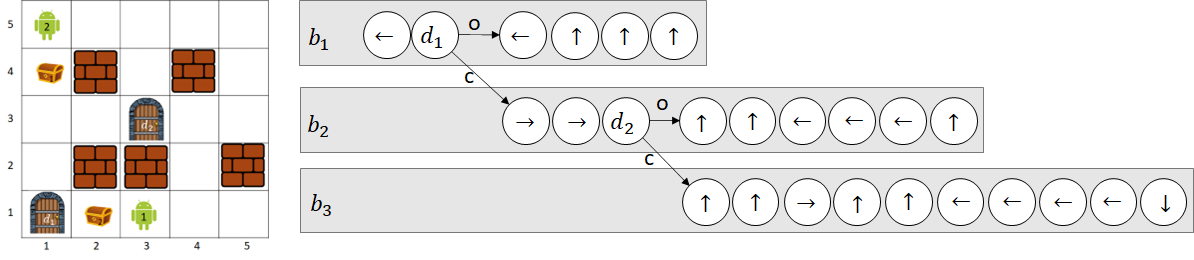
\includegraphics[scale=.28]{Figures/ExampleAndPlanTree.png}
      \caption{Example grid. Agents must reach their designated treasure boxes. Doors can be open or closed. A possible plan tree for agent 1. Arrows denote moving actions. $d_i$ denotes sensing whether door $i$ is open. $o,c$ denote open and closed.}
    \label{fig:Example}
\end{figure}
\commentout{
\begin{figure}[t]
    \begin{subfigure}[b]{0.5\textwidth}
    \centering
      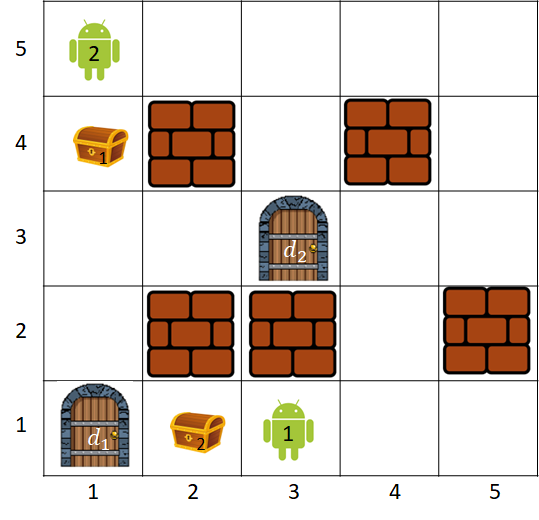
\includegraphics[scale=.2]{Figures/Example5x5.png}
      \caption{Example grid. Agents must reach their designated treasure boxes. Doors can be open or closed.}
    \end{subfigure}\quad
    \begin{subfigure}[b]{0.5\textwidth}
      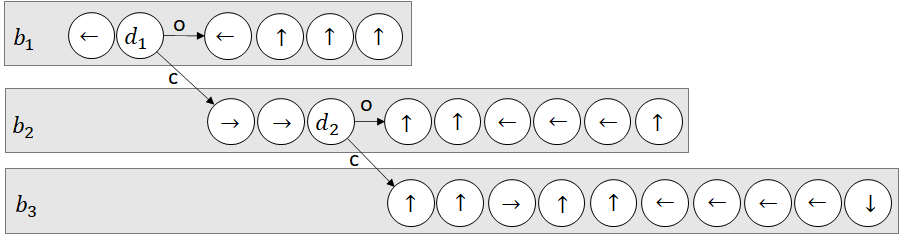
\includegraphics[scale=.25]{Figures/PlanTree.png}
      \caption{A possible plan tree for agent 1. Arrows denote moving actions. $d_i$ denotes sensing whether door $i$ is open. $o,c$ denote open and closed.}
      \label{fig:PlanTree}
    \end{subfigure}
    \caption{Running example.}
    \label{fig:Example}
\end{figure}
}
\subsubsection{Conflict Resolution}
Once a conflict between several agents has been identified, it must be resolved to ensure a safe solution. Given a conflict between a subset of agents, we can plan jointly for the subset, avoiding joint actions that lead to a collision \cite{standley2010finding}. However, planning for multiple agents together increases the problem complexity exponentially. Thus, such methods scale up poorly.
The \emph{conflict based search} (CBS) \cite{sharon2015conflict} algorithm employs a different conflict resolution method in which constraints are introdued over the set of vertices an agent can visit at a given time. We denote by $\langle i,v,t \rangle$ a constraint on agent $i$ not to visit $v$ at time $t$.
We can then use standard pathfinding algorithms to solve individually for each agent subject to these the constraints. To ensure optimality, when two agents $i,j$ have a potential conflict on vertex $v$ at time $t$, we can create two possible constraints $\langle i,v,t \rangle$ and $\langle j,v,t \rangle$. We can then solve once for each constraint, replanning only for the agent that received the constraint. We can then observe the two solutions, and choose the one that is better, e.g., with a lower sum of costs.
As there can be multiple conflicts, CBS maintains a set of constraints on each agent, and can be considered to search the space of possible constraint sets. This search process can be maintained as a binary tree, called the \emph{constraint tree}.
\subsubsection{Contingent Planning}
In classical automated planning agents fully observe the current state. In contingent planning under partial observability \cite{albore2009translation,BrafmanS12,bonet2011planning} some aspects of the problem are hidden, but can be either directly observed using sensing actions, or reasoned about given some observations.
A solution to such problems can be formalized as a plan tree, or more compactly, a plan graph \cite{muise2014computing,MaliahKS21}.
A common approach to computing such plan graphs is to plan until the next sensing action, and then replan following each possible observation \cite{bonet2011planning,MaliahKS21}. Extensions to multiple agents where also suggested \cite{brafman2013qualitative,bazinin2018iterative} in a decentralized setting.
The MAPFOU problem that we suggest here can be modeled as a contingent planning problem (for centralized execution), or as a multi-agent QDec-POMDP (for decentralized execution). However, current contingent solvers support much more complicated settings, such as complex relationships between the unobserved aspects, and as such, do not scale as well. One may consider our suggested approach as a domain specific adaptation of replanning-based contingent solvers, scaling to much larger problems.
The concept of optimal plan trees is also not trivial. It is unclear how one can aggregate over multiple branches to compare plan trees. Averaging over branches makes the underlying assumption of uniform distribution. As the probability of obstacle existence is unknown, any such assumption may lead to unjustified preference over plan trees \cite{shmaryahu2019comparative}. In this paper we focus on either optimizing for the best case, i.e., when all obstacles are absent, or for the worst case, where all obstacles exist. We make no guarantees over other plan tree branches.
Our problem is also related to the Canadian Traveler Problem (CTP)~\cite{papadimitriou1991shortest,bnaya2009canadian}, a shortest path problem where some edges are blocked with some probability. In MAPFOU, however, we do not have a probability distribution over the potentially blocked vertices.
\subsubsection{MAPF Variants with Uncertainty}
Various forms of uncertainty in MAPF were studies in the past.
In MAPF with delay probabilities (MAPF-DP) each agent action may be delayed with some probability \cite{wagner2017path,honig2016multi,atzmon2020probabilistic}. In stochastic MAPF
\cite{levy2022online} an agent may stochastically move in a different direction than intended.
Our problem is fundamentally different, as we do not assume known probabilities over the potential obstacles' state.
MAPF variants under known stochastic uncertainty were also suggested.
Atzmon et al.'s~\shortcite{atzmon2020robust} work on robust MAPF finds solutions to CMAPF problems that are robust to delays up to  a fixed threshold.
Shahar et al.~\shortcite{shahar2021safe} explored MAPF with time uncertainty (MAPF-TU), given a lower and upper bound over action duration. They proposed both an offline approach and an online approach, and distinguished between free and limited communication, as we do.
They did not propose an offline solution that is optimal and considers the observed information.
\section{Problem Definition}
We now describe an extension to MAPF that we call \emph{multi-agent path finding under obstacle uncertainty} (MAPFOU). In MAPFOU, a subset of vertices in the graph may be blocked by obstacles. We call these vertices \emph{potential obstacles} (\pos). The \emph{state} of a \po is either \emph{blocked} or \emph{unblocked}.
The agents do not initially know the state of the potential obstacles, but can use sensing actions to reveal them.
More formally, a MAPFOU problem is a tuple $\langle G,s,t,O\rangle$,
where $G,s,t$ are as in a CMAPF problem and $O \subseteq V$ is the set of \pos.
An \emph{obstacle configuration} $c:O\rightarrow\{\blocked, \unblocked, \unknown\}$ is a mapping between \pos and their possible state.
We included here an artificial state $\unknown$, to enable representing incomplete knowledge of a \po's state.
We say that an obstacle configuration $c$ is \emph{complete} if every \po is mapped to either \blocked\ or \unblocked, i.e., there is no \po $p$ such that $c(p)=\unknown$.
We say that two \pos $c$ and $c'$ are \emph{consistent}, denoted $\cons(c,c')$ if they agree on the state of every \po they know about, i.e.,
\begin{equation}
    \forall p\in O: c(p)=c'(p)\vee c(p)=\unknown \vee c'(p)=\unknown
    \label{eq:consistent}
\end{equation}
In our setting, there is a single obstacle configuration that is true and does not change throughout the execution. That is, \pos are either blocked or unblocked even before the agents start moving, and obstacles do not appear or disappear throughout the execution. The solver, of course, does not initially know the true obstacle configuration.
The set of actions of an agent in a MAPFOU problem contains the move and wait actions of a CMAPF problem, as well as \emph{sense} actions for each $v \in O$.
In this paper, we assume that sensing actions can only be executed when the agent is near an obstacle. That is, an agent located at vertex $v_i$ can observe the occurrence of obstacle in $v_j$ only if there exists an edge $(v_i, v_j) \in E$. That being said, this problem setting can be extended to remote sensing, although other algorithms may be needed for such settings.
A single-agent plan in a MAPFOU problem is a plan tree $\tau$, where nodes are labeled by actions, and edges are labeled by observations. For move and wait actions, there is a single outgoing edge labeled by the $null$ observation. For sense actions, there are two outgoing edges labeled $\blocked(v)$ and $\unblocked(v)$, where $v$ is the sensed vertex.
A node $n$ in the tree is associated with a vertex $n.v \in V$ and a time step $n.t$, which are the position of the agent in the graph and the time step, respectively, when it reaches $n$.
Each node $n$ in the plan tree is also associated with a partial obstacle configuration $n.K$, representing the agent's knowledge about the state of the potential obstacles when it reaches $n$. In our sensing model, $n.K$ corresponds to the set of potential obstacles that were sensed on the path from the root to $n$.
\begin{exmp}
For the example in Figure~\ref{fig:Example}, the vertices of the $G$ are the grid cells, and edges denote neighboring cells. In this case movement actions correspond to moving from the current grid cell in one of the principal directions.
Doors here, that may be open or closed, correspond to the possible obstacles. That is, $O=\{ \langle 1,1 \rangle, \langle 3,3 \rangle \}$.
Figure~\ref{fig:Example} also shows an example of a plan tree. Nodes are labeled by actions, where arrows denote movement, and $d_i$ denote sensing actions over the vertex where $d_i$ resides. Each such sensing action can have two possible outcomes --- the doors is either open or closed, and hence, the vertex is either blocked or unblocked, respectively.
In this plan tree agent 1 first attempts to move through door $d_1$. If it observes, once it is near the door, that the door is open, it moves up towards its treasure box (branch $b_1$). If $d_1$ is closed, it attempts to go to door $d_2$, to move through it to the box ($b_2$). If that door is closed as well, the agent is forced to go around the walls ($b_3$).
\end{exmp}
To generalize the notion of a conflict, we observe that a
branch in a single-agent plan tree $\tau$ represents a classical single-agent plan. Formally, for a single-agent plan tree $\tau$ and an obstacle configuration $c$, we denote by $\toplan(\tau,c)$ the classical single-agent plan represented by the corresponding branch in $\tau$.
\begin{definition}[Conflict between Plan Trees]
A pair of plan trees $\tau^i$ and $\tau^j$ has a conflict if there exists a complete obstacle configuration $c$
for which the classical single-agent plans $\toplan(\tau^i,c)$ and $\toplan(\tau^j,c)$ have a conflict.
\label{def:conflicting-plan-trees}
\end{definition}
A  MAPFOU solution is a set of plan trees, one per agent. For every leaf node $n$ of $\tau^i$, $n.v=t_i$ and there are no conflicts between its constituent single-agent plan trees.
\subsubsection*{Objective Function}
We assume that sensing actions do not have an inherent cost, and only consider the cost of the agents move and wait actions.
Following prior work on MAPF with non-deterministic delays~\cite{shahar2021safe}, we consider two alternative objective functions: \emph{best-case} SOC and \emph{worst-case} SOC.
This also conforms with solution cost measures that have been proposed for single-agent plan trees \cite{shmaryahu2019comparative}.
Let $SOC(\{\pi^i\})$ denote the SOC of a set of classical single-agent plans $\{\pi^i\}$, and let $\mathcal{C}(\mathcal{P})$ denote all possible obstacle configurations for a MAPFOU problem $\mathcal{P}$:
\begin{eqnarray}
 \mbox{best-case SOC: } \min_{c\in\mathcal{C}(\mathcal{P})} SOC(\{\toplan(\tau^i,c)\}) &&\\
 \mbox{worst-case SOC: } \max_{c\in\mathcal{C}(\mathcal{P})} SOC(\{\toplan(\tau^i,c)\})&&
\end{eqnarray}
\begin{observation}
For any MAPFTOU problem $\mathcal{P}$, if $\{\tau^i\}$ is an optimal solution wrt
the best-case SOC objective function then its cost is equal to the SOC of the single-agent plans corresponding to the obstacle configuration where all potential obstacles are \unblocked.
Similarly, the optimal worst-case SOC is equal to the SOC of the single-agent plans corresponding to the obstacle configuration where all potential obstacles are \blocked.
\label{obs:best-and-worst}
\end{observation}
\begin{algorithm}[t]
\caption{Centralized execution, best case}
    \label{alg:CEBC}
\footnotesize
\SetKwBlock{CEBC}{CEBC}{end}
\SetKwBlock{Main}{Main}{end}
\SetKwInOut{Input}{Input: }
\SetKwInOut{Output}{Output: }
\CEBC{
\Input{Graph $G$, Start vertices $S$, Target vertices $T$}
\Input{Obstacle configuration $K$, Unknown \pos $U$}
    $G' \leftarrow \assumeObs\left(G, K\cup \{v: \unblocked | v\in U\}\right)$\\
    $\{\pi^1,\ldots,\pi^k\} \leftarrow \textbf{PlanCMAPF}(G',S,T)$ \nllabel{cebc:plancmapf}\\
    \ForEach{agent $i$}{
        $(n^i_1,\ldots n^i_{|\pi^i|})\gets\textbf{CreateBranch}(\pi^i)$
    }
    \For{$j=1...\max(|\pi^i|)-1$}{
        Find $p\in U$ such that $p \notin K\wedge \exists i : \langle p, n^i_{j}.p \rangle \in E$\\
        \If{there exists such $p$}{
            $\{\tau'^i \} \leftarrow CEBC\left(G, [n^i_j.p]_i, T,
            K \cup \{p:\blocked\},U \setminus\{p\}\right)$ \\
            \For{every agent $\ell$}{ % $k$ is the number of agents so changed to \ell
                Add a new node $n_{sense}$ with action $Sense(p)$ before $n^\ell_j$\\
                Add an outgoing edge from $n_{sense}$, marked $unblocked(p)$, with child $n^\ell_j$\\
                Add an outgoing edge from $n_{sense}$, marked $blocked(p)$, with child $\tau'^\ell$\\
            }
            Add $p:\unblocked$ to $K$\\
            Remove $p$ from $U$
        }
    }
    For every agent $i$, create plan tree $\tau^i$, with root $n^i_1$\\
    \Return{$\{ \tau^i \}$}
}
\Main{
    CEBC$(G,s,t,\emptyset, O)$
}
\end{algorithm}
\subsubsection*{Centralized vs. Decentralized Execution}
We assume planning is centralized, and consider two possible execution paradigms: \emph{centralized} and \emph{decentralized}. In centralized execution, agents constantly share their observations and coordinate the actions. That is, when one agent senses a potential obstacle, all agents are immediately notified of the outcome of this sensing action. Then, an agent can branch its plan tree based on observations of other agents.
In decentralized execution, communication during execution is prohibited, and each agent must rely only on its own observations.
It is also possible that communication has costs, and agents must decide whether to sense themselves, or obtain information from other agents. We leave this for future research.
In summary, we consider in this work four variants of the MAPFOU problem:
Centralized Execution while optimizing for the Best Case SOC (CEBC),
Centralized Execution while optimizing for the Worst Case SOC (CEWC),
Decentralized Execution while optimizing for the Best Case SOC (DEBC), and
Decentralized Execution while optimizing for the Worst Case SOC (DEWC).
\section{Solving MAPFOU Using Replanning}
We now present a set of algorithms for finding optimal solutions for all the MAPFTO variants we consider in this work.
\subsection{Centralized Execution}
For the MAPFOU centralized execution variants (CEBC or CEWC), we propose an iterative approach in which the algorithm focuses on one obstacle configuration at a time, building the set of plan trees one branch at a time.
Observe that a MAPFOU with a single obstacle configuration is essentially a CMAPF problem.
We can use a standard CMAPF solver to solve this CMAPF problem, resulting in a set of safe single-agent plans for that particular obstacle configuration.
We convert each single-agent plan to a branch in the set of plan trees,
adding a sense action whenever an agent is adjacent to a potential obstacle that has not been sensed yet.
For each of these sense actions, we call again the CMAPF solver starting from the agent's expected location and the observation outcome that was not explored yet.
Algorithm~\ref{alg:CEBC} presents the psuedo code for our algorithm for CEBC variant (omitting some details for ease of exposition).
The input to our CEBC algorithm is
(1) $G$, the underlying graph of the MAPFOU problem,
(2) $S$, the currently assumed locations of the agents,
(3) $T$, the target location of the agents,
(4) $K$, an obstacle configuration representing an assumption over the state of some of the potential obstacles,
and (5) $U$, a set of potential obstacles whose state in not specified in $K$.
For a MAPFOU problem $\tuple{G,s,t,O}$ the initial call to our CEBC algorithm sets
$S=s$, $T=t$, $K=\emptyset$, and $U=O$, representing that the agents are in their initial locations and we do not assume anything yet about the the states of the potential obstacles.
We begin (line 2) by constructing an obstacle configuration that is consistent with $K$ and assumes all vertices in $U$ are unblocked.
Then we create a corresponding graph $G'$, removing all vertices that are considered blocked (the \assumeObs\ function), define a CMAPF problem $\tuple{G',S,T}$ and solve it using an off-the-shelf CMAPF solver  (the \textbf{PlanCMAPF} function).
This results in a conflict-free set of classical single-agent plans $\Pi=\{\pi^i\}$  (line 3). Each single-agent plan in this set is then transformed into a branch in the plan tree of the corresponding agent (line 4).
We then traverse these branches, searching for a the earliest node in which an agent is planned to occupy a vertex that is adjacent to a potential obstacle $p$ that was not sensed yet (line 7).
Then, we add a $Sense(p)$ action to all plan trees (line 12)  creating a branch in the plan trees to allow all agents to behaving differently depending on whether given that potential obstacle blocked or not.
In this, we abuse notation, as only one agent actually senses whether $p$ is blocked, and all other agents only observe the result.
We recursively create plan trees for the case where $p$ is blocked (line 10), and link the resulting trees following the sensing nodes (line 14).
Finally, we add the assumption that $p$ is unblocked to $K$ and remove it from $U$. Hence, if another agent must later pass through $p$, it no longer needs to sense whether it is blocked.
We ignore many details. For example, it might be that multiple agents pass through possibly blocked vertices at the same time step, requiring a more delicate, but straightforward, treatment with multiple consecutive sensing actions.
\begin{figure}[t]
    \begin{subfigure}[b]{0.4\textwidth}
      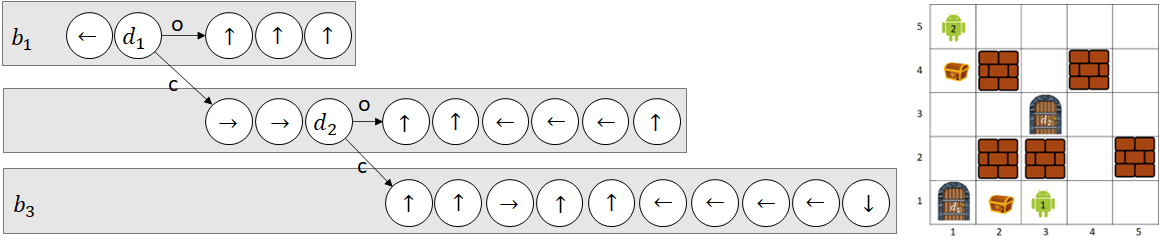
\includegraphics[scale=.25]{Figures/CEBC1+example.png}
      \caption{CEBC, Agent 1}\label{fig:CEBC1}
    \end{subfigure}
    \begin{subfigure}[b]{0.4\textwidth}
      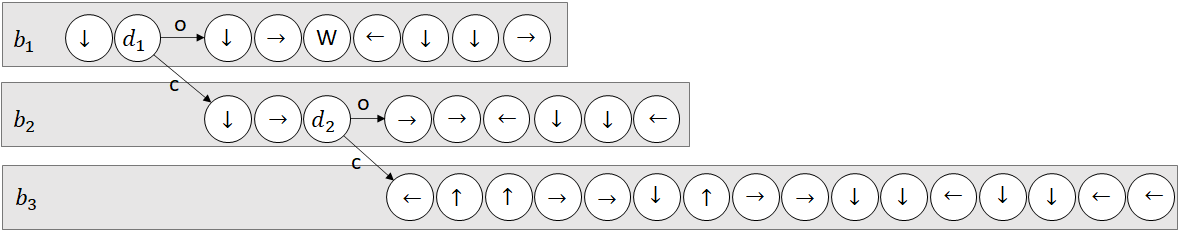
\includegraphics[scale=.25]{Figures/CEBC2.png}
      \caption{CEBC, Agent 2}\label{fig:CEBC2}
    \end{subfigure}
    \begin{subfigure}[b]{0.4\textwidth}
      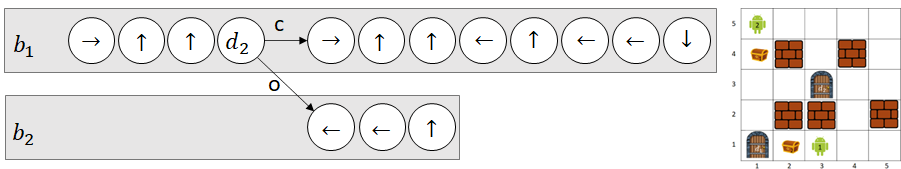
\includegraphics[scale=.25]{Figures/CEWC1+example.png}
      \caption{CEWC, Agent 1}\label{fig:CEWC1}
    \end{subfigure}
    \begin{subfigure}[b]{0.4\textwidth}
      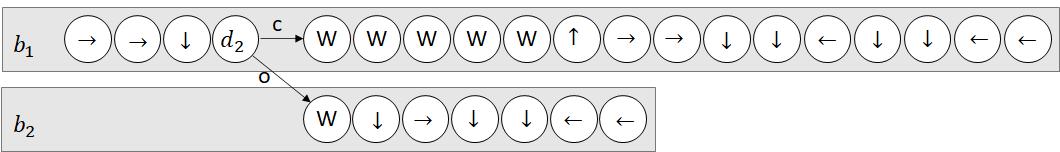
\includegraphics[scale=.25]{Figures/CEWC2.png}
      \caption{CEWC, Agent 2}\label{fig:CEWC2}
    \end{subfigure}
    \caption{Plan trees for centralized execution for the running example. Arrows denote movement actions, $W$ denotes waiting, $d_i$ denote sensing whether door $i$ is open or closed, $o,c$ denote the open and closed observations.}
\end{figure}
\begin{exmp}
Figures~\ref{fig:CEBC1} and ~\ref{fig:CEBC2} show the plan trees created by CEBC. We first call CEBC with $K=\emptyset$, $U=\{d_1,d_2\}$,  the agent start positions: $s_1=\langle 3,1 \rangle$, $s_2=\langle 1,5 \rangle$, and the agent target positions, where the boxes are located: $t_1=\langle 1,4 \rangle$, $t_2=\langle 2,1 \rangle$.
First, assuming doors are open, the CMAPF solver generates (lines 3-5) the topmost branches ($b_1$ in both trees) , without the sensing action ($d_1$). The CMAPF solver has identified a conflict, and resolved it by moving agent 2 to the side and waiting for agent 1 to get to its target. Then, agent 2 can move to its own target.
After moving left in the first action, agent 1 can sense as to whether $d_1$ is open. As observations are shared during the central execution, we add the sensing action in both plan trees (line 12), allowing agent 2 to act differently if $d_1$ is closed. When $d_1$ is closed, we call CEBC recursively (line 10), with $K=\{blocked(d_1)\}$, and $U=\{d_2\}$, and $S$ is the current position of the agents: $s_1=\langle 2,1 \rangle$, and $s_2=\langle 1,4 \rangle$. Now, it is beneficial for both agents to try and pass through $d_2$. Agent 2 moves to the left of $d_2$, and senses. Then, again, we branch in both trees. We call CEBC recursively with $K=\{blocked(d_1),blocked(d_2)\}$, $U=\emptyset$, $s_1=\langle 4,1 \rangle$, and $s_2=\langle 2,3 \rangle$.
\end{exmp}
\commentout{
\begin{algorithm}[t]
\caption{Centralized Execution, Worst Case (CEWC)}
    \label{alg:CEWC}
\footnotesize
\SetKwBlock{CEWC}{CEWC}{end}
\SetKwInOut{Input}{Input: }
\SetKwInOut{Output}{Output: }
\CEWC{
\Input{Grid $G$, Known obstacles $K$, Unknown obstacles $U$, Start positions $S$, Target positions $T$}
    $G' \leftarrow $ A grid identical to $G$ where all vertices in $U$ are blocked, and all vertices in $K$ are as observed\\
    $\Pi \leftarrow PlanCMAPF(G',S,T)$\\
    For every agent $i$, create a sequence of nodes $n^i_j$ corresponding to the vertices in $\pi^i$, marking all edges using the null observation\\
    $K' \leftarrow \emptyset$\\
    \For{$j=1...\max(|\pi^i|)-1$}{
        Find $p$ s.t. $p \in U \setminus K', \exists i : \langle p, n^i_{j}.p \rangle \in E$\\
        \If{there exists such $p$}{
            $\{\tau^k \} \leftarrow SEBC(G,K \cup \{blocked(p'):p' \in K'\} \cup \{unblocked(p)\},U \setminus (K' \cup \{p\}), \{n^l_j.p : \textrm{for every agent } l\}, T)$ \roni{Shouldn't this be CEWC and not SEBC?}\\
            \For{every agent $k$}{
                Add a new node $n_{sense}$ with action $Sense(p)$ before $n^k_j$\\
                Add an outgoing edge from $n_{sense}$, marked $blocked(p)$, with child $n^k_j$\\
                Add an outgoing edge from $n_{sense}$, marked $unblocked(p)$, with child $\tau^k$\\
            }
            Add $p$ to $K'$\\
        }
    }
    For every agent $i$, create plan tree $\tau^i$, with root $n^i_1$\\
    \Return{$\{ \tau^i \}$}
}
\end{algorithm}
}
Optimizing for the worst case, i.e., when all obstacles are assumed to be blocked, is very similar. CEWC (centralized execution worst case) differs from CEBC (Algorithm~\ref{alg:CEBC}) in that we assume in the CMAPF problem (line 2) that all unobserved vertices are blocked. The recursive call (line 9), assumes that $p$ is unblocked, allowing a possible shortcut over the worst case. The children of the sensing nodes are also attached to the opposite case than in CEBC.
\begin{exmp}
Figures~\ref{fig:CEWC1} and ~\ref{fig:CEWC2} show the plan trees for the worst case. Here, we assume that all doors are closed. Hence, the CMAPF solver must move the agents around the doors, with a long wait (denoted $W$) for agent 2 until agent 1 moves past the conflict area. It happens that here both agents move next to $d_2$ --- agent 1 on its shortest path, and agent 2 as it needs to move aside allowing agent 1 to pass. Then, one agent can sense for $d_2$, and if it happens to be open, both agents can design a shorter path (branch $b_2$).
We can see that for our running example, as often happens in our experiments, the worst case avoids possible obstacles, and thus the plan trees have less branches. For plan cost, we can see that the best case in CEBC has a sum of costs of 12 (ignoring sensing), and 16 for CEWC. For the worst case, the sum of costs is 32 in CEBC, and 29 in CEWC.
\end{exmp}
We use our own implementation of CBS, using $A^*$ as the internal planner, to solve the CMAPF problems.
\begin{theorem}
Given a sound, complete, and optimal CMAPF solver, CEBC and CEWC algorithms are also sound, complete, and optimal, i.e., guaranteed to return a solution, if such exists, which has no conflicts and is optimal wrt to the chosen objective function (best- or worst-case SOC).
\end{theorem}
\begin{proof}
\noindent \textbf{Soundness.}
Every branch in the plan trees returned by our algorithm is created by running a CMAPF solver under the assumption of a specific obstacle configuration for all agents.
As the CMAPF solver is sound, the branches of the plan trees do not contain any conflict, and all agents end at the goal in that branch. In addition, the main loop (lines 6-15) ends after inspecting all actions in the active branch, and hence the plan tree does not contain any unexplored branches.
Thus, the solution is sound, i.e., conflict-free and in all leaves, all agents reached their target.
\noindent\textbf{Completeness.}
As the underlying graph $G$ is undirected and sensing actions do not change it, the agents can always backtrack to any joint state they occupied before. Thus, adding nodes and edges to the plan trees never results in a dead-end.
The number of potential obstacles in finite and every recursive call to our algorithm removes one potential conflict from $U$. Hence, we are a guaranteed that our algorithm terminates in finite time.
\noindent\textbf{Optimality.} Consider the the best-case SOC objective function. We know that the optimal best-case SOC is equal to the solution of the CMAPF problem that corresponds to assuming all potential obstacles are unblocked (Observation~\ref{obs:best-and-worst}). By construction, our algorithm is guaranteed to include that solution as branches in the resulting set of plan trees.
\end{proof}
\subsection{Decentralized Execution}
\label{scn:decentralized}
For decentralized execution, agents do not share their observations, and hence, different plan trees branch on different observations.
We thus take a different approach, inspired by the CBS algorithm~\cite{sharon2015conflict}.
First, each agent computes a complete plan tree ignoring all other agents. We take an approach similar to CEBC (Algorithm~\ref{alg:CEBC}), using a single-agent solver ($A^*$) instead of a CMAPF solver (line~\ref{cebc:plancmapf}) to generate single-agent plans.
Then, we search for possible conflicts between these plan trees.
If a conflict is detected, we resolve it by imposing
constraints on each of the conflicting agents, and replan their plan trees accordingly.
\subsubsection{Conflict Detection}
\label{scn:conflicts}
One may detect conflicts between plan trees $\tau^i$ and $\tau^j$ by enumerating all possible complete obstacle configurations $c\in\mathcal{C}(\mathcal{P})$, checking for conflicts between the corresponding single agent plans $\toplan(\tau^i,c)$ and $\toplan(\tau^j,c)$.
We suggest a more efficient method.
\begin{definition}[Conflict between Plan Tree Nodes]
A pair of plan tree nodes $n^i\in\tau^i$ and $n^j\in\tau^j$ for agents $i$ and $j$ (where $i\neq j$), respectively, form a conflict if
(1) $n^i.v = n^j.v$,
(2) $n^i.t = n^j.t$,
and (3) $n^i.c$ and $n^j.c$ are consistent.
\label{def:mapfou-conflict}
\end{definition}
That is, a pair of nodes $\tuple{n^i,n^j}$ from different plan trees form a conflict if they represent the same location and time, and their obstacle configurations are consistent.
We can connect Definition~\ref{def:conflicting-plan-trees} (tree conflict) and  Definition~\ref{def:mapfou-conflict} (node conflict).
\begin{observation}
Plan trees $\tau^i$ and $\tau^j$ have a conflict
iff there exists two nodes $n^i\in\tau^i$ and $n^j\in\tau^j$ that form conflict.
\label{obs:conditionsForConflicts}
\end{observation}
In decentralized execution, we check if a pair of plan trees has a conflict by searching for a pair of nodes in them that form a conflict, i.e., reside in non-conflicting branches.
This conflict detection method can be much more efficient than iterating over all obstacle configurations.
\subsubsection{Conflict Resolution}
\label{scn:conflicts-resolution}
CBS resolves conflicts by imposing constraints of the form $\tuple{i,v,t}$, representing that agent $i$ cannot visit vertex $v$ at time $t$. In our case, however, a conflict formed by a pair of nodes  at vertex $v$ and time $t$ is only relevant under the respective nodes' obstacle configurations.
Therefore, the constraint we use to resolve a conflict formed by a pair of plan-tree nodes must include  information about the obstacle configurations where it is relevant.
We define the following type of MAPFOU constraint:
\commentout{
\begin{definition}[MAPFOU Constraint]
A MAPFOU constraint is defined by a tuple $\tuple{i,v,t,c_i,c_j}$
where $i$ is an agent,
$v$ is a vertex,
$t$ is a time step,
and $c_i$ and $c_j$ are obstacle configurations.
A plan tree $\tau$ satisfies a MAPFOU constraint if one of the following conditions holds:
\begin{eqnarray}
(C1) ~~~ \forall p\in O&:& \left(c(p)=c_i(p)\right)\vee \left(c(p)=\unknown\right) \\
(C2) ~~~ \forall p\in O&:& c_i(p)\neq\unknown \rightarrow c(p)=c_i(p) ~ \wedge  \\
 &&   c_i(p)=\unknown \rightarrow c(p)=c_j(p)
\end{eqnarray}
\label{def:mapfou-constraint}
\end{definition}
To understand Definition~\ref{def:mapfou-constraint}, consider a conflict formed by a pair of plan tree nodes
$n^i\in\tau^i$ and $n^j\in\tau^j$ at vertex $v$ and time $t$ with obstacle configurations $c_i$ and $c_j$, respectively.
A plan tree $\tau$ for agent $i$ does not satisfy the MAPFOU constraint $\tuple{i,v,t,c_i,c_j}$ if and only if
it includes a node $n$ that has the agent in $v$ at time $t$ in an obstacle configuration that either is on the plan tree branch leading to $n^i$ (condition C1) or on a plan tree branch after $n^i$ that is consistent with $c_j$ and only sensed additional \pos (over $c_i$) that were sensed by $c_j$.
To ensure optimality, we follow the same framework as CBS, where both options to resolve any identified conflict are checked. This is managed by maintaining a constraint tree in which each node represents a set of plan trees and a set of constraints. A best-first search over this tree on the desired objective function is guaranteed to be sound, complete, and optimal following the same proof as in the original CBS.
\begin{theorem}
DEBC is sound, complete, and optimal.
\label{the:debc-optimal}
\end{theorem}
The proof, as well as an example, can be found in the supplementary material.
\commentout{
\begin{proof}
Soundness is guaranteed because only solutions without conflicts are returned.
To prove completeness and optimality in the same way given for the standard CBS-based algorithms~\cite{sharon2015conflict,atzmon2020robust,li2020new}, we must prove that the pair of constraints we impost when a conflict is detected is \emph{sound}~\cite{atzmon2020robust,li2020new}.
That is, the constraints we impose do not preclude reaching any (conflict-free) solution.
To see this, consider a conflict formed by a pair of plan tree nodes
$n^i$ and $n^j$ at vertex $v$ and time $t$ with obstacle configurations $c_i$ and $c_j$, respectively.
The corresponding MAPFOU constraints are $\tuple{i,v,t,c_i,c_j}$
and $\tuple{j,v,t,c_j,c_j}$.
We will now show that any solution to the given MAPFOU solution must satisfy at least one of these constraints.
We prove this by negation: let $\{\hat{\tau}^i\}$ be a (conflict-free) solution that does not satisfy both constraints.
This means the plan trees $\hat{\tau}^i$ and $\hat{\tau}^j$
include nodes
$\hat{n}^j$ and
$\hat{n}^i$, respectively,
where $\hat{n}^i.v=v$, $\hat{n}^i.t=t$,
and $\hat{n}^i.c$ and $\hat{n}^j.c$
satisfy either (C1) or (C2) from Definition~\ref{def:mapfou-constraint}
for their respective constraints.
Thus, either both nodes satisfy (C1), both satisfy (C2), or one satisfies (C1) and the other (C2).
For each of these cases, $\hat{n}^i.c$ and $\hat{n}^j.c$ ends up being consistent, which means that $\hat{n}^i$ and $\hat{n}^j$ form a conflict, contradicting the assumption that $\{\hat{\tau}^i\}$ is a (conflict-free) solution.
\end{proof}
}
The above conditions and constraint-tree search are not trivial to implement. Thus, in our implementation we simplified in two ways.
First, we only considered condition (C1) and not (C2). This does not hinder completeness or optimality, but may cause the constraint tree to have more nodes.
Second, we searched the constraint tree greedy search instead of a best-first search. This does have implications on completeness and optimality. Yet, we observed almost no quality reductions in our experiments.
}
\begin{definition}[MAPFOU Constraint]
A MAPFOU constraint is defined by a tuple $\tuple{i,v,t,c_i,c_j}$
where $i$ is an agent,
$v$ is a vertex,
$t$ is a time step,
and $c_i$ and $c_j$ are obstacle configurations.
A plan tree $\tau$ for agent $i$ violates this MAPFOU constraint if there exists a node $\hat{n}\in\tau$ where $\hat{n}.v=v$,  $\hat{n}.t=t$, and for every $p\in O$ the following conditions holds
\begin{eqnarray}
\left(c_i(p)\neq\unknown\right)\rightarrow \left(\hat{n}.c(p)=c_i(p)\vee \hat{n}.c(p)=\unknown\right) \label{eq:root-to-node}
\\
\left(c_i(p)=\unknown\right)\rightarrow \left(\hat{n}.c(p)=c_j(p)\vee \hat{n}.c(p)=\unknown\right)  \label{eq:node-to-leaf}
\end{eqnarray}
\label{def:mapfou-constraint}
\end{definition}
Intuitively, the first condition (Equation~\ref{eq:node-to-leaf}) ensures that the obstacle configuration of $\hat{n}$ is on the same branch in the plan tree as $c_i$,
and the second condition (Equation~\ref{eq:node-to-leaf}) ensures that
if $\hat{n}$ is deeper than $n^i$ in the plan tree then every \pos it sensed is consistent with $c_j$.
To ensure optimality, we follow the same framework as CBS, where both options to resolve any identified conflict are checked. This is managed by maintaining a constraint tree in which each node represents a set of plan trees and a set of constraints. A best-first search over this tree on the desired objective function is guaranteed to be sound, complete, and optimal following the same proof as in the original CBS.
\begin{theorem}
DEBC is sound, complete, and optimal.
\label{the:debc-optimal}
\end{theorem}
The proof, as well as an example, can be found in the supplementary material.
\commentout{
\begin{proof}
Soundness is guaranteed because only solutions without conflicts are returned.
To prove completeness and optimality in the same way given for the standard CBS-based algorithms~\cite{sharon2015conflict,atzmon2020robust,li2020new}, we must prove that the pair of constraints we impost when a conflict is detected is \emph{sound}~\cite{atzmon2020robust,li2020new}.
That is, the constraints we impose do not preclude reaching any (conflict-free) solution.
To see this, consider a conflict formed by a pair of plan tree nodes
$n^i$ and $n^j$ at vertex $v$ and time $t$ with obstacle configurations $c_i$ and $c_j$, respectively.
The corresponding MAPFOU constraints are $\const_i=\tuple{i,v,t,c_i,c_j}$
and $\const_j=\tuple{j,v,t,c_j,c_j}$.
Assume by negation that $\{\hat{\tau}^i\}$ is a (conflict-free) solution that violates $\const_i$ and $\const_j$.
This means the plan trees $\hat{\tau}^i$ and $\hat{\tau}^j$
include nodes
$\hat{n}^j$ and
$\hat{n}^i$, respectively,
where $\hat{n}^i.v=v$, $\hat{n}^i.t=t$,
and for every $p\in O$
$\hat{n}^i.c$ and $\hat{n}^j.c$
satisfy the conditions in Equations~\ref{eq:root-to-node} and~\ref{eq:node-to-leaf} for every $p\in O$.
Since we assumed $\{\hat{\tau}^i\}$ a conflict-free solution,
this means $\hat{n}^i.c$ and $\hat{n}^j.c$ cannot be consistent.
By definition of consistency (Equation~\ref{eq:consistent}), this means
there exists $\pbad\in O$ sensed in both obstacle configurations
$\hat{n}^i.c$ and $\hat{n}^j.c$ where the sensed state was different.
Since $n^i$ and $n^j$ formed a conflict, $c_i$ and $c_j$ must be consistent.
Thus, if $\pbad$ was sensed by $c_i$ and $c_j$,
then they agree on its state (i.e., $c_i(\pbad)=c_j(\pbad)$).
Due to Equation~\ref{eq:root-to-node}, this means $\hat{n}^i.c$ and $\hat{n}^j.c$ must also agree on $\pbad$'s state.
Alternatively, assume without loss of generality that $\pbad$ was not sensed by $c_i$ (i.e., $c_i(\pbad)=\unknown$).
Due to Equation~\ref{eq:node-to-leaf}, this means $\hat{n}^i.c$ must agree with $c_j$ and $\hat{n}^j.c$ on $\pbad$'s state.
Thus contradicting the assumption that $\{\hat{\tau}^i\}$ is a conflict-free solution.
\end{proof}
}
The above conditions and constraint-tree search are not trivial to implement.
Thus, in our implementation we simplified in two ways.
First, we only considered the condition in Equation~\ref{eq:node-to-leaf} when considering MAPFOU constraints. This does not hinder completeness or optimality, but may cause the constraint tree to have more nodes.
Second, we searched the constraint tree with a greedy search instead of a best-first search.
This does have implications on completeness and optimality.
Yet, we observed almost no quality reductions in our experiments.
\roni{Issues to raise:
1) This constraint is different from not allowing the agent to be at $v$ and $t$ all along the branch. Doing this is, I believe, incomplete.
2) This constraint is also different from replanning from the root up to the brach. Because, sometimes the branching may change. In other words, the plan tree my branch in different ways, after multiple replans. For example, one plan tree may branch first on obstacle $p1$ while after several replanning it might choose to branch first over obstacle $p2$. I am almost certain this can happen.}
\section{Empirical Evaluation}
We now discuss a set of experiments, designed to shed light on the properties of the various approaches that we suggest. Our methods are implemented in Java. Experiments were run on a an $i7$, 2.8GHz CPU, with 16GB RAM, but only 4GB were used.
In the experiments below we use $A^*$ for computing optimal paths, and our implementation of conflict resolution. We did not use an off-the-shelf CMAPF solver.
\subsubsection{Benchmark Domains}
In our experiments, we follow the MAPF community \cite{stern2019multi}, defining grids of various sizes and properties. In our grids, aside from the start and target locations of the agents, we also add a set of grid cells that may contain obstacles, placing them at strategic points in the grid, while ensuring that there is always a path between any two cells, even if all obstacles exist.
We experiments on two types of grids --- room grids, where the space is split into rooms with one cell doorways, and open grids, with a few known obstacles, and a number of possible obstacles.
We use two different grid sizes.
\commentout{
To create benchmark MAPFOU problems, we use standard problems from the MAPF community \cite{}. All problems are defined on grid settings.
A classical MAPF problem is defined by a graph (grid) and a set of $k$ source and target vertices. Corresponding to that, a benchmark domain for MAPF includes a set of graphs.
\\We evaluated our methods on two general benchmark domains that are commonly used:
\begin{itemize}
  \item \textbf{Open N × N grids with random obstacles}. These are N × N grids, where all grid cells are accessible but a set of grid cells that are randomly selected and are considered to be impassable (static obstacles).
  \plan{TODO insert image}
  \item \textbf{Room Grid-Based MAPF}. These are N x N Grids, that are divided for same sized rooms. Each rooms has at least one "door" - accessible empty cell on the border of the room that lead to another room. Two or more doors from a given room can lead to the same room or to different rooms.
\plan{TODO insert image}
\end{itemize}
\plan{new experiments with A* - MA}
\\Another set of experiments that we executed is comparison between our method to classic A* for multi-agent settings. In multi-agent A* a node is represented a state of all agents' locations, and an edge is existing iff it doesn't cause for conflicts and iff the transition for each agent between the two vertices location is legal. We would like to examine the improvement of our method against the classical state-of-the-art solution
}
\subsubsection{Protocol}
For each of the grid types, we generate 10 test problems. Given $k$, the number of agents, we randomly choose for each agent a start and target position in the grid. In a grid with $N$ predefined possible obstacle positions, given $n\leq N$, the number of obstacles in the test problem, we randomly choose $n$ of the possible obstacles positions, assuming the rest of the possible obstacles do not exist.
Below, we report average results over the 10 executions.
When testing scaling up, we set a time limit of 15 minutes for a given experiments. We limit our experiments to cases where all 10 problems were solved within the given time.
\commentout{
\plan{Methods}
\\As mentioned in previous section, we ran 4 sets of experiments:
\begin{enumerate}
  \item \textbf{Sensitivity analysis - increasing agents amount} - In this set of experiments we took a 32x32 grid and static amount of suspected obstacles. In each experiment in this set the only setting that changed is the amount of agent (in each instance the actual obstacles location has chosen randomly as described above).
  \item \textbf{Sensitivity analysis - increasing obstacles amount} - In this set of experiments we took a 32x32 grid and static amount of agents. In each experiment in this set the only setting that changed is the amount of obstacles (in each instance the actual agents source and target locations has chosen randomly as described above).
  \item \textbf{Sensitivity analysis - increasing grid size} - In this set of experiments we took static amount of agents and suspected obstacles. In each experiment in this set the only setting that changed is the the grid size. The grid type remained the same (room type or open grid with random obstacles)
  \item \textbf{Comparison to naive solution} - In this set of experiments evaluate and compared between our method to state-of-the-art multi-agent A* on the same identical problems.
\end{enumerate}
\plan{best-worst, with/without communication}
\\We ran the sensitivity analysis on all modes and approached presented on this paper:
\begin{itemize}
  \item No communication with best case optimization (room typed grid). \item No communication with best case optimization (open grid).
  \item No communication with worst case optimization (room typed grid).
  \item With communication with worst case optimization (open grid).
  \item With communication with best case optimization (room typed grid).
  \item With communication with best case optimization (open grid).
  \item With communication with worst case optimization (room typed grid).
  \item With communication with worst case optimization (open grid).
\end{itemize}
We ran the comparison to Multi-Agent A* on the settings of No communication with best-case optimization on room-typed grid
}
\subsubsection{Results}
First, we implemented a solver over the joint space of all agents. In this case a search space node consists of the positions of all agents. Actions are joint, that is, all possible combinations of movements of all agents. We eliminate actions that lead to a collision, and hence a single search is sufficient, and there is no need for conflict detection and resolution. The joint solver plans for one branch at a time, similar to CEBC and CEWC.
\begin{table}[t]
\centering
\scriptsize
\begin{tabular}{| c | c | c | r | r |}
\hline
Grid & Agents & Obstacles & Joint & DEBC \\ \hline
$6 \times 6$ & 3   & 2 & 2.400 & 0.027 \\ \hline
$8 \times 8$ & 3   & 2 & 313.780 & 0.041 \\ \hline
$13 \times 13$ & 2   & 3 & 11.400 & 0.140 \\ \hline
$15 \times 15$ & 2   & 3 & 39.830 & 0.200 \\ \hline
$17 \times 17$ & 2   & 3 & 133.330 & 0.300 \\ \hline
\end{tabular}
\caption{Comparing runtime (sec) between solving the joint problem, and our DEBC solver.}
\label{tbl:joint}
\end{table}
Table~\ref{tbl:joint} shows the results. Clearly, the joint space grows exponentially, and we cannot handle problems with more than 2-3 agents and 2-3 obstacles, even for small grids.
Figures~\ref{fig:GridSizeOpen} and ~\ref{fig:GridSizeRoom} show the runtime as the grid grows. As expected, the runtime grows exponentially with the grid size. The runtime in open grids grows faster than for room grids. This is because in open grids, when agents take the shortest path, their paths intersect much more often, and the amount of conflict resolutions grows, requiring more time to resolve. This is more pronounced in the centralized execution case, as agents branch on observations from other agents, over obstacles that they do not necessarily pass through.
\begin{figure}[t]
    \centering
    \begin{subfigure}[b]{0.2\textwidth}
      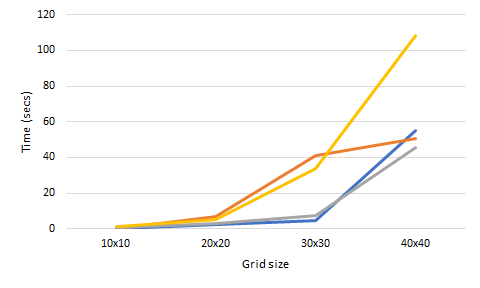
\includegraphics[scale=.27]{Figures/GridSizeOpen.png}
      \caption{Open, increasing grid size, 3 agents, 5 obstacles}
      \label{fig:GridSizeOpen}
    \end{subfigure}
    \begin{subfigure}[b]{0.2\textwidth}
      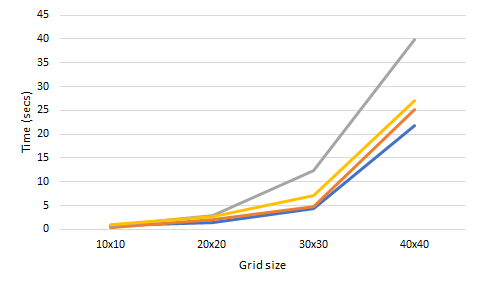
\includegraphics[scale=.27]{Figures/GridSizeRoom.png}
      \caption{Room, increasing grid size, 3 agents, 5 obstacles}
      \label{fig:GridSizeRoom}
    \end{subfigure}
    \begin{subfigure}[b]{0.2\textwidth}
      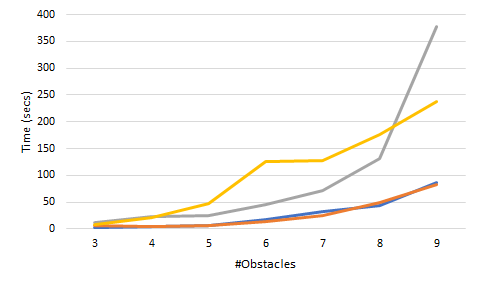
\includegraphics[scale=.27]{Figures/ObstaclesTimeOpen32.png}
      \caption{Open, $32\times 32$, increasing obstacles, 7 agents}
      \label{fig:ObstaclesOpen}
    \end{subfigure}
    \begin{subfigure}[b]{0.2\textwidth}
      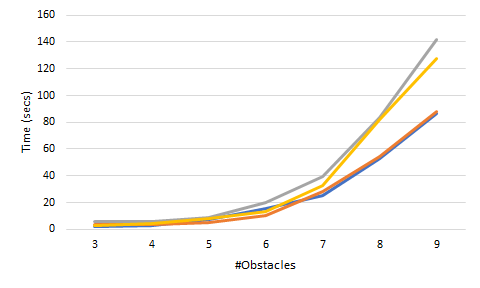
\includegraphics[scale=.27]{Figures/ObstaclesTimeRoom32.png}
      \caption{Room, $32\times 32$, increasing obstacles, 7 agents}
      \label{fig:ObstaclesRoom}
    \end{subfigure}
    \begin{subfigure}[b]{0.2\textwidth}
      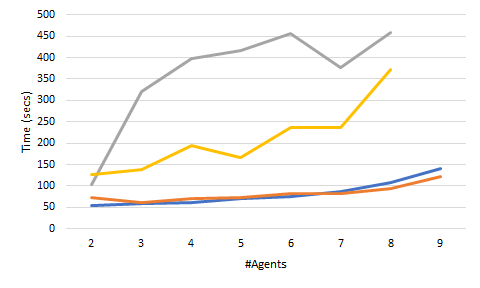
\includegraphics[scale=.27]{Figures/AgentsTimeOpen32.png}
      \caption{Open, $32\times 32$, increasing agents, 9 obstacles}
      \label{fig:AgentsOpen}
    \end{subfigure}
    \begin{subfigure}[b]{0.2\textwidth}
      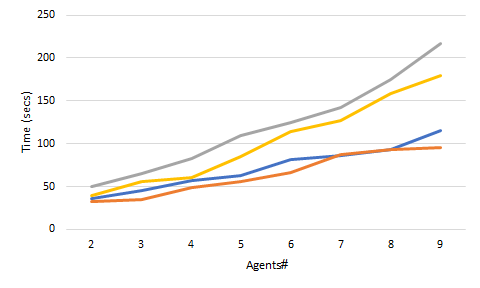
\includegraphics[scale=.27]{Figures/AgentsTimeRoom32.png}
      \caption{Room, $32\times 32$, increasing agents, 9 obstacles}
      \label{fig:AgentsRoom}
    \end{subfigure}
        \begin{subfigure}[b]{0.24\textwidth}
      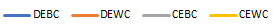
\includegraphics[scale=.5]{Figures/LegendHorizontal.png}
    \end{subfigure}
    \caption{Comparing execution time}
    \label{fig:32}
\end{figure}
We now analyze our algorithm sensitivity to the number of agents and obstacles.
Figure ~\ref{fig:32} compares the run time  increases. As we can see (Figures~\ref{fig:ObstaclesOpen} and ~\ref{fig:ObstaclesRoom}), increasing   in the plan tree, which requires replanning for exponentially more branches. Again, centralized execution results in splitting over observations that are not necessarily relevant. This is most obvious in the open environment, where movement is less restricted, and hence less obstacles are relevant for an agent.  An interesting future research, would allow agents to ignore observations that are not relevant for them.
When increasing the amount of agents (Figures~\ref{fig:AgentsOpen} and \ref{fig:AgentsRoom}) the increase is almost linear for the distributed execution case. This is due to our distributed computation, where we create plan trees for each agent independently. As these grids are fairly large, with respect to the number of agents, conflicts do not happen too often. Here, centralized planning over the open grid presents the toughest problems to solve, and with 9 agents, both CEBC and CEWC failed to solve the problem within the 15 minutes timeout. This is because in the open grid most obstacles are not relevant for most agents, yet reporting them requires substantial additional planning.
\commentout{
\begin{table*}
\tiny
\begin{tabular}{|l||l|l||l|l||l|l|l||l|l|l||l|l|l|l||l|l|l|l|}
\hline
& \multicolumn{4}{c||}{2 agents}& \multicolumn{6}{c||}{3 agents}& \multicolumn{8}{c|}{4 agents} \\ \hline
	&	\multicolumn{2}{c|}{DEBC-CEBC}	&			\multicolumn{2}{c||}{DEWC-CEWC}		&			\multicolumn{3}{c||}{DEBC-CEBC}	&					\multicolumn{3}{c||}{DEWC-CEWC}		&					\multicolumn{4}{c||}{DEBC-CEBC}			&					\multicolumn{4}{c|}{DEWC-CEWC}	 \\ \hline
Conf	&	A1	&	A2	&	A1	&	A2	&		A1	&	A2	&	A3	&	A1	&	A2	&	A3	&		A1	&	A2	&	A3	&	A4	&	A1	&	A2	&	A3	&	A4	\\ \hline
0000	&	2	&		&		&		&			&	2	&		&		&		&		&			&	2	&		&	2	&		&		&		&		\\ \hline
0001	&	2	&		&		&		&			&	2	&		&		&	-2	&	2	&			&	2	&		&	2	&		&		&		&		\\ \hline
0010	&	2	&		&		&		&			&	2	&		&		&		&		&			&	2	&		&	2	&		&		&		&		\\ \hline
0011	&		&		&		&		&			&	2	&		&	2	&	-2	&	-2	&			&	2	&		&	2	&		&		&		&		\\ \hline
0100	&	2	&		&	4	&		&			&		&		&		&	-2	&	2	&			&		&		&		&	 	&		&		&		\\ \hline
0101	&		&		&	4	&	-2	&			&		&		&	2	&	-2	&	8	&			&		&		&		&	-2	&	2	&		&	2	\\ \hline
0110	&		&		&	4	&		&			&		&		&		&		&		&			&	2	&		&		&		&	2	&		&	2	\\ \hline
0111	&		&		&	4	&		&			&		&		&	2	&	-2	&	8	&			&		&		&		&		&	2	&		&	2	\\ \hline
1000	&	2	&		&		&		&			&	2	&		&		&		&		&			&	2	&		&	2	&		&		&		&		\\ \hline
1001	&	2	&		&		&		&			&	2	&		&		&		&		&			&	2	&		&	2	&		&		&		&		\\ \hline
1010	&	2	&		&		&		&			&	2	&		&		&		&		&			&	2	&		&	2	&		&		&		&		\\ \hline
1011	&		&		&		&		&			&	2	&		&	2	&		&		&			&	2	&		&	2	&		&		&		&		\\ \hline
1100	&		&		&	4	&		&			&		&		&		&		&	6	&			&		&		&		&		&	2	&		&	2	\\ \hline
1101	&		&		&	4	&	-2	&			&		&		&		&		&	6	&			&		&		&		&	-2	&	2	&		&	2	\\ \hline
1110	&		&		&	4	&		&			&		&		&		&		&	6	&			&		&		&		&		&	-2	&		&	-2	\\ \hline
1111	&		&		&	4	&		&			&		&		&	2	&		&	6	&			&		&		&		&		&	2	&		&	2	\\ \hline
\end{tabular}
\caption{Cost analysis \guy{need explanations here}}
\label{tbl:costs}
\end{table*}
\begin{table}
\tiny
\begin{tabular}{|l||l|l||l|l||l|l|l||l|l|l||l|l|l|l||l|l|l|l|}
\hline
& \multicolumn{4}{c||}{2 agents}& \multicolumn{6}{c||}{3 agents}& \multicolumn{8}{c|}{4 agents} \\ \hline
	&	\multicolumn{2}{c|}{Best}	&			\multicolumn{2}{c||}{Worst}		&			\multicolumn{3}{c||}{Best}	&					\multicolumn{3}{c||}{Worst}		&					\multicolumn{4}{c||}{Best}			&					\multicolumn{4}{c|}{Worst}	 \\ \hline
Conf	&	1	&	2	&	1	&	2	&		1	&	2	&	3	&	1	&	2	&	3	&		1	&	2	&	3	&	4	&	1	&	2	&	3	&	4	\\ \hline
0000	&	2	&		&		&		&			&	2	&		&		&		&		&			&	2	&		&	2	&		&		&		&		\\ \hline
0001	&	2	&		&		&		&			&	2	&		&		&	-2	&	2	&			&	2	&		&	2	&		&		&		&		\\ \hline
0010	&	2	&		&		&		&			&	2	&		&		&		&		&			&	2	&		&	2	&		&		&		&		\\ \hline
0011	&		&		&		&		&			&	2	&		&	2	&	-2	&	-2	&			&	2	&		&	2	&		&		&		&		\\ \hline
0100	&	2	&		&	4	&		&			&		&		&		&	-2	&	2	&			&		&		&		&	 	&		&		&		\\ \hline
0101	&		&		&	4	&	-2	&			&		&		&	2	&	-2	&	8	&			&		&		&		&	-2	&	2	&		&	2	\\ \hline
0110	&		&		&	4	&		&			&		&		&		&		&		&			&	2	&		&		&		&	2	&		&	2	\\ \hline
0111	&		&		&	4	&		&			&		&		&	2	&	-2	&	8	&			&		&		&		&		&	2	&		&	2	\\ \hline
1000	&	2	&		&		&		&			&	2	&		&		&		&		&			&	2	&		&	2	&		&		&		&		\\ \hline
1001	&	2	&		&		&		&			&	2	&		&		&		&		&			&	2	&		&	2	&		&		&		&		\\ \hline
1010	&	2	&		&		&		&			&	2	&		&		&		&		&			&	2	&		&	2	&		&		&		&		\\ \hline
1011	&		&		&		&		&			&	2	&		&	2	&		&		&			&	2	&		&	2	&		&		&		&		\\ \hline
1100	&		&		&	4	&		&			&		&		&		&		&	6	&			&		&		&		&		&	2	&		&	2	\\ \hline
1101	&		&		&	4	&	-2	&			&		&		&		&		&	6	&			&		&		&		&	-2	&	2	&		&	2	\\ \hline
1110	&		&		&	4	&		&			&		&		&		&		&	6	&			&		&		&		&		&	-2	&		&	-2	\\ \hline
1111	&		&		&	4	&		&			&		&		&	2	&		&	6	&			&		&		&		&		&	2	&		&	2	\\ \hline
\end{tabular}
\caption{Cost analysis \guy{need explanations here}}
\label{tbl:costs}
\end{table}
}
\begin{figure}[t]
\centering
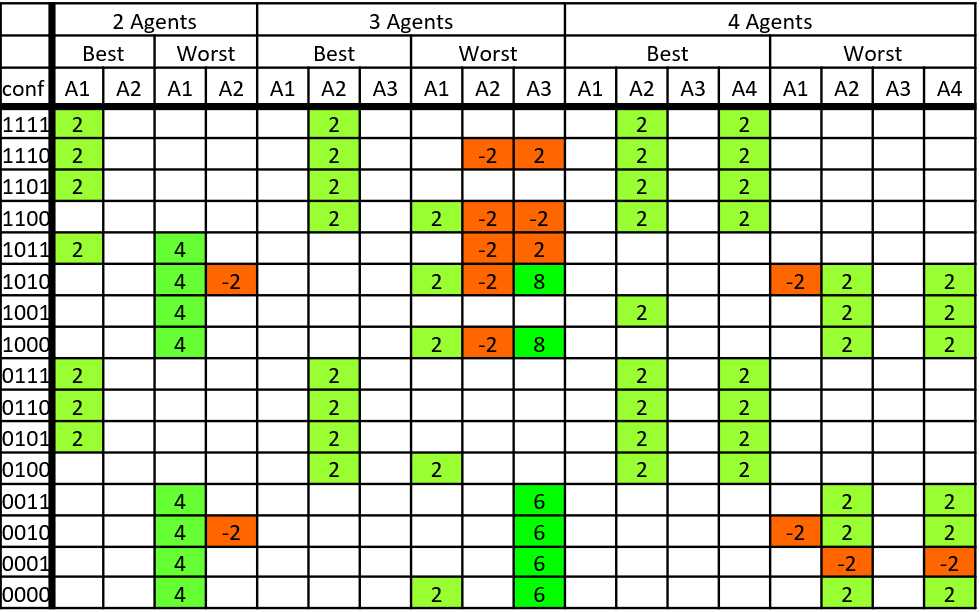
\includegraphics[scale=.4]{Figures/CostTable.png}
      \caption{Difference between centralized and decentralized execution costs. Conf denotes obstacle configuration. 1 denotes unblocked. 0 denotes blocked. $A_i$ denotes agent $i$.}
      \label{fig:CostTable}
\end{figure}
We now analyze the benefits of using a centralized execution, where agents share information about the observed obstacles. For the best and worst case that we focus on here, there is no difference, because for the best case all obstacles are missing, while for the worst case, all obstacles exist. As this is what the planner assumes, receiving information about the obstacles does not modify the extreme plans. However, differences may occur in other branches.
For analyzing these costs differences in branches other than the best and worst case, we used a smaller, $12\times 12$ grid, with 4 obstacles, and vary the amount of agents. Figure~\ref{fig:CostTable} shows the difference between the centralized and decentralized execution, when there is a difference. With 2 agents, many obstacles are not relevant for one of the agents, and sharing information does not help. In one case  information about an unblocked cell, for the worst case optimization, caused agent 1 to use a substantially shorter path.
For 3 agents, we get more pronounced differences. Agent 3 can save 6-8 actions when it gets information from other agents. For 4 agents, the differences are much smaller, be  choose. Hence, information about obstacles is less helpful.
\section{Conclusion}
In this paper we suggest a new variant of multi agent path finding, called MAPFOU, assuming that some vertices may be blocked. We provide formal definition for the new problem and its solution. We suggest two optimization criteria, focusing on the best and worst case. We suggest methods for two alternatives --- when information about observed obstacles is communicated, and when no communication is allowed. We show in our experiments how our methods scale up given the grid size, number of agents, and the amount of unknown obstacles.
We believe that MAPFOU opens the path for many research questions. Future research can focus on handling problems with communication costs, on ignoring irrelevant obstacles in centralized execution, on handling other types of conflicts, on remote sensing, and much more.
Dolore eum molestiae amet ab illum optio fuga ipsam, exercitationem quia ex rem expedita vero eligendi facere molestias, expedita provident nihil aliquid impedit rerum laudantium reiciendis maiores corporis sunt, enim voluptas ratione magnam soluta dolores id deleniti eligendi, aliquid iure placeat inventore veritatis soluta cupiditate adipisci quam unde esse culpa.\clearpage
\bibliography{aaai23}
\end{document}